\documentclass{arima-en}
% force arXiv/HAL to compile with PDFLaTeX
\pdfoutput=1 

%%%%%%%%%%%%%%%%%%%%%%%%%%%%%%%%%%%%%%%%%%%%%%%%%%%%%%%
% Modules
\usepackage{array}
\usepackage{pgfplots}
\usepackage{graphicx}
\usepackage[utf8]{inputenc}
\usepackage[T1]{fontenc}
\usepackage{fancyhdr}
\pagestyle{fancy}
\usepackage{hyperref}
\usepackage[babel]{csquotes}
\usepackage{acronym}

%%%%%%%%%%%%%%%%%%%%%%%%%%%%%%%%%%%%%%%%%%%%%%%%%%%%%%%
% Header
\title{Prédiction du risque de crédit bancaire en intégrant des descripteurs extraits des graphes multicouches}
\author[1]{Victor Nico DJIEMBOU TIENTCHEU}
\author[1,2,3]{Armel Jacques NZEKON NZEKO'O}
\author[1,2,3]{Maurice TCHUENTE}
\affil[1]{Université de Yaoundé I, Département d’Informatique, BP 812, Yaoundé, Cameroun} 
\affil[2]{Fondation pour la Recherche, l’Ingénierie et l’Innovation, FR2I, BP 14306, Yaoundé, Cameroun} 
\affil[3]{Sorbonne Université, IRD, UMI 209 UMMISCO, F-93143, Bondy, France}


% corresponding author with his/her email
\corrauthor{nico.djiembou@facsciences-uy1.cm}

%%%%%%%%%%%%%%%%%%%%%%%%%%%%%%%%%%%%%%%%%%%%%%%%%%%%%%%
%Code for software citations
\usepackage[
  style=numeric-comp,
  datamodel=software, % extend the datamodel with entries for software
  abbreviate=false,
  natbib=true,
  sorting=ynt,
  backend=biber,
  bibencoding=utf8,
  giveninits=true,
  url=false,
  doi=false,
  defernumbers,
  maxcitenames=10,
  defernumbers=false,
  maxbibnames=100]{biblatex}
%
% Load the software biblatex style
%

\usepackage{software-biblatex}
%
% Set software specific bibliography options
%
\ExecuteBibliographyOptions{
  halid=true,
  swhid=true,
  swlabels=true,
  vcs=true,
  license=false}
%
% Make title an hyperlink to the DOI or URL to make the result leaner (suggested by N. Rougier 4/4/2020)
%

\newcommand{\doiorurl}{%
 \iffieldundef{doi}
    {\iffieldundef{url}
       {}
       {\strfield{url}}}
    {http://dx.doi.org/\strfield{doi}}%
}
\newcommand{\myhref}[1]{%
 \ifboolexpr{%
  test {\ifhyperref}
  and
  not test {\iftoggle{bbx:url}}
   and
   not test {\iftoggle{bbx:doi}}
  }
  {\href{\doiorurl}{#1}}
  {#1}%
}
\DeclareFieldFormat{title}{\myhref{\mkbibemph{#1}}}
\DeclareFieldFormat
  [article,inbook,incollection,inproceedings,patent,thesis,unpublished]
  {title}{\myhref{\mkbibquote{#1\isdot}}}
\addbibresource{references.bib}

% Définition des acronymes
\acrodef{IA}{Intelligence Artificielle}
\acrodef{AA}{Apprentissage Automatique}
\acrodef{MLN}{MultiLayer Network}
\acrodef{PME}{Petites et Moyennes Entreprises}
\acrodef{ANN}{Artificial Neural Network}
\acrodef{RNN}{Recurrent Neural Network}
\acrodef{LSTM}{Long Short-Term Memory}
\acrodef{DT}{Decision Tree}
\acrodef{LR}{Logistic Regression}
\acrodef{XGB}{eXtreme Gradient Boosting}
\acrodef{SVM}{Support Vector Machine}
\acrodef{RF}{Random Forest}
\acrodef{SCF}{Supply Chain Finance}
\acrodef{HARA}{Hub Authority Ranking Applicants Algorithm}
\acrodef{HubAvgRA}{Hub-Avg ranking applicants Algorithm}
\acrodef{ATkRA}{Authority-Threshold Algorithm}

% retirer les acronyms du document.
%%%%%%%%%%%%%%%%%%%%%%%%%%%%%%%%%%%%%%%%%%%%%%%%%%%%%%%
\pgfplotsset{compat=1.17}
\begin{document}
\maketitle





%%%%%%%%%%%%%%%%%%%%%%%%%%%%%%%%%%%%%%%%%%%%%%%%%%%%%%%
\abstract {
% contexte
% texte conci
Le prêt est l'une des principales sources d'enrichissement des banques, mais est également une source de perte financière. Pour optimiser leurs profits, il est donc nécessaire pour les banques de prédire si un emprunteur remboursera ou pas son crédit. 
% transition vers IA
Afin d'aider les banques à aborder efficacement ce challenge, plusieurs techniques d'apprentissage automatique ont été proposées durant cette dernière décennie pour la question spécifique de prédiction du risque de crédit bancaire. 
% transition vers graphe
Quelques unes de ces techniques reposent sur des graphes  
% transition vers graphes mutlicouches 

% limites actuelles du graphe multicouche 

% travaux réalisé pour palier les limites 

% description de l'environnement d'expérimentation, jeu de données, modèles considérés, métriques d'évaluation, ...

% remarques et résultats intéressants 


L'amélioration de la capacité de ses institutions à évaluer le risque associé à une demande de prêt a été confronté à des difficultés parmi lesquelles la faible présence de données pour entraîner les modèles d'\ac{AA} et la faible représentativité dans les jeux de données existant. L'analyse des comportements des emprunteurs et des liens avec leur entourage au moyen de modèles graphes a été longtemps utiliser pour augmenter les jeux de données existant avec des informations pertinentes pour combler le manque de données et relativement leur représentativité. 

% objectif
Ainsi de nombreux travaux en \ac{IA} ont réussi jusqu'ici à proposer un moyen d'analyser les emprunteurs suivant deux dimensions. Différentes paires d'attributs catégorielles sont prise de façon aléatoire dans l'ensemble d'informations et sont modélisé au moyen de graphes multicouches biparti où chaque couche met les emprunteurs en relations avec la valeur d'attribut associée constituant cette couche. Ensuite des informations pertinentes comme le PageRank avec une personnalisation inter-couche, intra-couche et collective de ces graphes sont calculées via l'analyse de graphes. Néanmoins, l'aléa dans le choix d'attributs du jeu données, la limite du nombre de dimension et encore la limitation au attributs catégorielles constituent une limite car de façon hypothétique, je suis en relation avec un ensemble d'individu parce que je partage au moins une information avec cette ce groupe. 
% méthodologie
Alors, pour résoudre ses limites, nous adaptons d'abord l'algorithme de PageRank personnalisé multicouche pour prendre en compte unique les informations propres à un seul emprunteurs lors de la recherche d'information pertinente, ensuite nous proposons un protocole qui permet de choisir les k attributs à utiliser dans un graphe multicouche biparti à k couches, enfin les informations extraites sont intégrées dans des modèles \ac{AA} notamment afin d'améliorer les métriques de classification de ses modèles. 
% resultats
Nous l'avons approuvé à 5 jeux de données benchmark dans le domaine du credit scoring et avons observé que nous améliorons les résultats présentent dans la littérature.
% contributions
% implications
% Conclusion
}
\keywords{risque de crédit, graphe, graphe multicouche}
%\ac{IA}; \ac{AA}; analyse de graphes; Finances et économie; Risque de Crédit;}
% risque de crédit, graphe, graphe multicouche


%%%%%%%%%%%%%%%%%%%%%%%%%% 
% je me dis qu'il faut un état de l'art sur l'usage des modèles de machine learning dans la prédiction du risque de crédit de façons générale pour justifier le choix des modèles choisis.

% deuxièmement, un etat de l'art sur l'usage des structures de graphes pour répresenter et analyser les liens complexes entre les transactions

% troisièmement, faire une petit rappel memoire de quelques notions dans la théorie des graphes 
%%%%%%%%%%%%%%%%%%%%%%%%%%

%%%%%%%%%%%%%%%%%%%%%%%%%%%%%%%%%%%%%%%%%%%%%%%%%%%%%%%
\section{Introduction}

%%%%%%%%%%%%%%%%%%%%%%%%%%%%
%%%%%%%%% Credit scoring Context
D’après la publication du 25/01/2023 de “\textit{la finance pour tous}”\cite{tous_credit_2023}, bien que l’importance relative du crédit dans le financement de l’économie a reculé par rapport aux financements réalisés via les marchés financiers, le crédit reste l’un des mécanismes fondamentaux de la vie économique et de la croissance. Toutefois, faire crédit c’est prendre des risques de non remboursement, de liquidité, de taux d’intérêt qui sont étroitement liés aux comportements des emprunteurs et de leur entourage. Alors avec la crise financière du subprime de 2008\cite{tous_crise_2024}, de nombreuses recherches se sont proposées pour améliorer la l’économie dans le monde via l’\ac{AA}.

%%%%%%%%% MLNA context
Dans une ère où les modèles graphes sont au coeur de l'\ac{IA}, l'apprentissage basé sur les modèles graphes a longtemps fait ses preuves dans la résolution de ses problèmes du secteur de l'économie et la finance. Cependant son fort coût temporel et spatial est ce facteur qui à permet de faire émerger l'analyse de graphes qui au lieu de faire un apprentissage sur les graphes vise plutôt à extraire des motifs ou informations complexe dans des graphes au service des modèles d'\ac{AA}. Cette dernière de part sa complexité réduite a été sujet à de nombreuse utilisation sur de nombreux modélisation en graphes parmi lesquels la modélisation en graphes multicouche biparti qui se considère comme un moyen de mieux capturer les relations nivelées entre emprunteurs dans un réseau. 

%%%%%%%%%%% Problem
Ainsi donc depuis la crise des subprimes en 2008, un intérêt particulier a été porté à la mitigation du risque de crédit moyennant diverses approches, finance comportementale, l'évaluation des actifs, la réglementation financière, la modélisation des risques, la gestion des risques, les marchés financiers, la macroéconomie, la politique monétaire et la gouvernance d'entreprise. La gestion des risques en particulier s'est intéressée à l'évaluation de nombreux risques dont celui des risques de crédit avec pour objectif de réduire l'impact négatif des risques et de maximiser les opportunités. 

%%%%%%%%%%%% state of art
Cette évaluation du risque de crédit financiers dans les banques a connu un grand avancement avec les méthodes d'analyse de graphe et d'\ac{AA}. les modèles d'\ac{AA} tels que \ac{SVM}, \ac{LR}, \ac{DT},\ac{RF}, \ac{XGB} ou encore d'apprentissage profond tels que \ac{ANN}, \ac{LSTM}, \ac{RNN} ont impacté positivement dans cette recherche par leur explicabilité et puissance d'analyse respectivement. Par contre, les modèles d'\ac{AA} et aussi les modèles d'apprentissage profond ont comme limite respective la forte dépendance à la qualité de données d'entraînement et la complexité temporelle et spatiale.

Alors dans une logique de pouvoir augmenter la quantité et la qualité de données utile au processus d'apprentissage, des mécanismes d'extraction de motifs pertinents des graphes ont été étudié sur plusieurs types de graphes,
% ...

C'est Face à ce couplage de besoin d'explicabilité et prise en compte des relations entre emprunteurs qu'une nouvelle vague de contribution naquit, celle de l'usage de la puisse de représentation des entités en structure graphe ou encore réseau. En effet, l'historique de transaction de prêt d'une institution financière peut être modélisé comme un réseau ou graphe dans lequel il est possible d'extraire les liens complexe. Cong Wang et Al.\cite{wang2021multiview} pour pouvoir prendre en compte les relations dans les \ac{SCF}, les situations de crédit des \ac{PME} et des entreprises principales dans l'évaluation du risque de crédit, ils vont proposer une méthode adaptative d’apprentissage de graphes  hétérogènes multivues pour le problème de la petite taille de l'échantillon à des fins de la prévision du risque de crédit des \ac{PME} dans un contexte avec des données non étiquetées. Leur approche à pour points fort de pouvoir répondre au problème d'absence de données étiquetées, capturer et intégrer l'importance de chaque vue du \ac{SCF} au profit du credit scoring. Cependant, cette approche est très coûteuse en temps et puissance de calcul, et sa performance dépend fortement de la qualité du graphe utilisé pour modéliser chaque vue de données issues de sources parfois différentes.

S. Mario\cite{mario2021graph} pour capturer les relations financières entre entités intervenantes (emprunteurs, instituts financiers) dans le contexte d’une inter-coopération des institutions financières et des emprunteur va modéliser un graphes orienté représentant une micro-structure du réseau où chaque noeud représente un emprunteur ou une institution financier et les arêtes, le lien financier existant entre les noeuds afin qu’au moyen de l'analyse de graphes, les informations de contagions ou tout autres relations complexe dans le réseau puissent être capturées et exploitées afin d’améliorer l’évaluation du risque de crédit avec des modèles explicable comme \ac{SVM} et \ac{LR}. Bien qu'améliorer l'évaluation avec des attributs pertinents extraits de graphes, il demeure vrai que l'accès à ce genre d'information est difficile et dont l'absence de ce genre de données rend l'approche difficile. Xiujuan Xu et Al.\cite{xu2009credit} vont construire un graphe biparti pour représenter les informations d'historique de prêts d'institut bancaire. Ici chaque noeud matérialise soit un emprunteur soit un modalité caractéristique et une arête entre un noeud emprunteur et un noeud modalité signifie que l'emprunteur est décrite par cette modalité. Pour prendre en compte les relations complexe entre les emprunteurs, ils vont utiliser trois algorithmes d'analyse de liens basés sur le prétraitement de \ac{SVM}: \ac{HARA}, \ac{HubAvgRA}, \ac{ATkRA}. Ses deux approches font bien d'utiliser des techniques d'analyse de graphes pour capturer des descripteurs pertinents pouvant améliorer la prédiction du risque de crédit par des algorithmes de machine learning classique, toutefois, analyser ses relations en considérant tous les caractéristiques comme étant la base absolu de leur relation n'est par raisonable. Intuitivement, si je suis en relation avec un individu c'est forcement au moins un niveau de caractérisation en commun mais oublier ce logique de niveau peut induire à l'extraction de fausse relations ou des relations de faible poids.

Mar{\'i}a {\'O}skarsd{\'o}ttir et Cristi{\'a}n Bravo\cite{oskarsdottir2021multilayer} tiennent compte du niveau de relation dans la modélisation du réseau d'emprunteur en utilisant des graphes multi-couches ou multiplexes (\ac{MLN}) biparti où chaque noeud d'une couche est soit un emprunteur soit une modalité de la dimension, chaque couche représente un niveau ou dimension d'analyse suivant une modélisation de graphe biparti et relié à la deuxième par le noeuds emprunteurs, les arêtes entre les noeuds emprunteurs et les noeuds de modalité représente la possession de cette modalité comme description de l'emprunteur pour cette dimension. Ils utilisent ensuite l'analyse de graphes pour capturer des relations entre emprunteurs dans les \ac{MLN} à k couches construites sur la base d'uplets (2-uplet) de attributs catégorielles prisent de manière aléatoire. Notamment, l'idée de PageRank à personalisation Intra-couche, Inter-couche et combinée semblent être capturer de très bonne relation. Cette approche bien que très intéressante pose certaines limites notamment, pourquoi ce limiter à ne manipuler que les attributs catégorielles pour définir les couches? comment choisir des attributs pertinentes pour la construction des couches de graphes multi-couches? ou encore 






%%%%%%%%%%%%%%%%%%%%%%%%%%%%%%%%%%%%%%%%%%%%%%%%%%%%%%%
\section{Related Work}
%%%%%%%%%%%%%%%%%%%%%%%%%%

\subsection{Théorie des graphes et la prédiction du risque de crédit}

%%%%%%%%%%%%%%%%%%%%%%%%%%
\subsection{Algorithmes d'apprentissage automatique pour la prédiction du risque de crédit financier}
%%%
\subsubsection{Arbre de décision (DT)}
\subsubsection{Regression Logistique (LR)}
\subsubsection{Forêt Aléatoire (RF)}
\subsubsection{eXtreme Gradient Boosting (XGBoost)}
Suspendisse vel dui nec felis molestie tincidunt. Vestibulum rutrum ligula lacus, ac molestie nulla fermentum ornare. Nulla non nunc euismod, porta lacus vestibulum, malesuada massa. Curabitur massa eros, rutrum sed lectus sed, volutpat semper metus. Mauris hendrerit aliquam commodo.  Vivamus fermentum tempus pellentesque. Maecenas a hendrerit urna. In elit ipsum, ultrices non dolor in, pulvinar porttitor lacus. Nunc euismod nibh quis odio condimentum, a feugiat massa rutrum. Nulla erat erat, adipiscing vitae lectus id, consectetur fermentum elit. Nunc eu est eu neque dapibus semper. Nam commodo urna dapibus, tincidunt turpis a, cursus sem. Vivamus venenatis adipiscing mollis. Cras fringilla sodales lobortis. Aliquam aliquet felis id est cursus auctor. Duis sodales tellus vulputate lectus egestas volutpat.





%%%%%%%%%%%%%%%%%%%%%%%%%%%%%%%%%%%%%%%%%%%%%%%%%%%%%%%
\section{Tables and Figures}
%%%%%%%%%%%%%%%%%%%%%%%%%%
\subsection{Tables}
Cf. Table~\ref{tab:example}.

\begin{table}
  \newcolumntype{+}{>{\global\let\currentrowstyle\relax}}
  \newcolumntype{^}{>{\currentrowstyle}}
  \newcommand{\rowstyle}[1]{\gdef\currentrowstyle{#1}%
    #1\ignorespaces
  }
  \centering
  \begin{tabular}{+>{\bfseries}l^c^c^c^c}
    \hline
    \rowstyle{\bfseries}
    & S-Length & S-Width & P-Length & P-Width\\
    Setosa & 5.006 & 3.428 & 1.462 & 0.246\\
    Versicolor & 5.936 & 2.77  & 4.26  & 1.326\\
    Verginica & 6.588 & 2.974 & 5.552 & 2.026\\
    \hline
  \end{tabular}
  \caption{Morbi malesuada diam at magna condimentum.}
  \label{tab:example}
\end{table}

\subsection{Figures}

If possible, bring figures together in a block. Use images at least 300 dpi. Check that caption are legible and in english. See this example : Figure~\ref{fig:example} (from  \url{http://www.texample.net/tikz/examples/pgfplots/}). The title must be ended with a dot.


%%%%%%%%%%%%%%%%%%%%%%%%%%
\begin{figure}
  \centering
  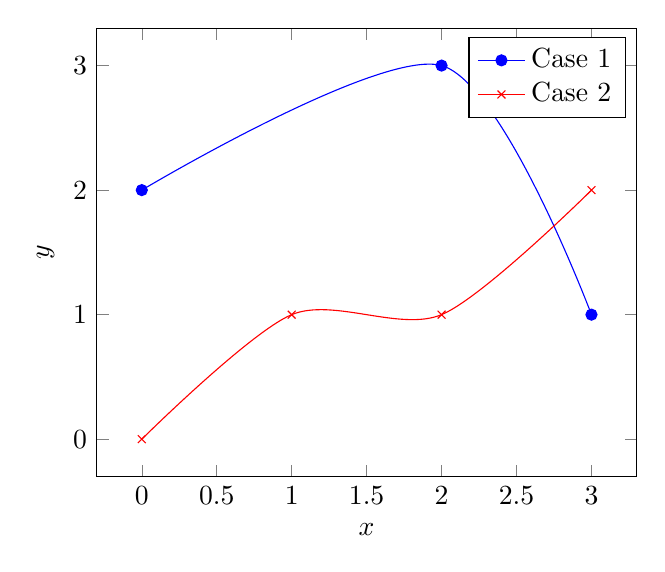
\begin{tikzpicture}
    \begin{axis}[
        xlabel=$x$,
        ylabel=$y$]
    \addplot[smooth,mark=*,blue] plot coordinates {
        (0,2)
        (2,3)
        (3,1)
    };
    \addlegendentry{Case 1}
    \addplot[smooth,color=red,mark=x]
        plot coordinates {
            (0,0)
            (1,1)
            (2,1)
            (3,2)
        };
    \addlegendentry{Case 2}
    \end{axis}
    \end{tikzpicture}
  \caption{figure de Christian Feuers\"anger; source: Pgfplots.}
  \label{fig:example}
\end{figure}

\begin{figure*}[ht] 
\resizebox{10cm}{9cm}
  {\includegraphics[width=11cm]{Lion.jpeg}}
  \centering
  \label{frog}
  \caption{Cameroon Lion (photo credit: Fist name Surname).}
  \end{figure*}
  




%%%%%%%%%%%%%%%%%%%%%%%%%%%%%%%%%%%%%%%%%%%%%%%%%%%%%%%
\section{Definitions, Algorithms and Formulas}
%%%%%%%%%%%%%%%%%%%%%%%%%%
\subsection{Definitions}
For formulas, use the package \texttt{amsthm} and the style \texttt{arima} for reliable formatting.

\begin{definition}[alpha]
Curabitur ullamcorper sit amet justo at hendrerit.
\end{definition}

Then we set the following definition.

\begin{definition}
Etiam sed nulla viverra, ultrices ligula ac, consectetur libero.
\end{definition}

For a list, use "bullets" or em dash:
\begin{itemize}
  \item Nunc id justo scelerisque ;
  \item metus id enim iaculis tristique.
\end{itemize}


%%%%%%%%%%%%%%%%%%%%%%%%%%
\subsection{Formulas}
Formulas Example:
\begin{equation}
  Y=M.^tM-\beta.\langle M \rangle_l
\end{equation}

where $\langle M \rangle_l$ is the mean vector of a $M$. $\beta$ enables the rate of close neighbours to be regulated.

Other formulas example:
\begin{equation}
  K * N_c = Cst \pm 0.001\%
\end{equation}


%%%%%%%%%%%%%%%%%%%%%%%%%%
\subsection{Algorithms}
For algorithms, use appearance of Algorithm~\ref{lst:example}. If necessary, see the package \texttt{listings}.

\begin{listing}
  \begin{lstlisting}
  partition(array, left, right)
     pivotIndex := choose-pivot(array, left, right)
     pivotValue := array[pivotIndex]
     swap array[pivotIndex] and array[right]
     storeIndex := left
     for i from left to right - 1
         if array[i] < pivotValue
             swap array[i] and array[storeIndex]
             storeIndex := storeIndex + 1
     swap array[storeIndex] and array[right]  // Move pivot to its final place
     return storeIndex
  \end{lstlisting}
  \caption{Partitioning function of a sorting algorithm.}
  \label{lst:example}
\end{listing}





%%%%%%%%%%%%%%%%%%%%%%%%%%%%%%%%%%%%%%%%%%%%%%%%%%%%%%%
\section{Conclusion and references}

%%%%%%%%%%%%%%%%%%%%%%%%%%
\subsection{Discussion}
Nam id eros massa. Fusce luctus purus a augue ullamcorper, sit amet vehicula mauris tristique. Suspendisse eget pulvinar odio, nec bibendum turpis. Nullam quis lectus porttitor, ullamcorper nisi et, condimentum leo. Quisque sed orci fermentum, rutrum velit eget, ultricies augue. Nunc porttitor consectetur tincidunt. Nulla tincidunt justo enim, vitae dignissim erat mattis ut. Nulla.


%%%%%%%%%%%%%%%%%%%%%%%%%%
\subsection{Conclusion}
Maecenas egestas metus id enim iaculis tristique. Etiam sed nulla viverra, ultrices ligula ac, consectetur libero. Nullam vitae massa ac odio pharetra condimentum. Maecenas in elementum libero, non gravida quam. Praesent adipiscing consectetur consectetur. Vivamus at orci sed augue varius hendrerit. Donec neque metus, dignissim nec erat at, ultricies consequat libero. Donec eget eleifend leo. Aliquam at nunc porta, mollis sapien eu, eleifend tortor. Nam egestas, metus ac pellentesque feugiat, lectus purus ornare est, vitae cursus felis turpis sit amet lacus. Donec consequat massa mi, ac suscipit arcu posuere et. Vivamus et semper risus. Sed ut arcu quam.

%%%%%%%%%%%%%%%%%%%%%%%%%%%%
% List of acronyms
%\printacronyms

%%%%%%%%%%%%%%%%%%%%%%%%%%%%%%%%%%%%%%%%%%%%%%%%%%%%%%%
%Code for bibliography with software 
\printbibheading
\printbibliography[heading=subbibliography,nottype=software,nottype=softwareversion,nottype=softwaremodule,nottype=codefragment,title={Publications}]
\printbibliography[heading=subbibliography,type=software,title={Software Project}]
\printbibliography[heading=subbibliography,type=softwareversion,title={Software versions, modules, excerpts and manuals}]
\nocite{*}


%%%%%%%%%%%%%%%%%%%%%%%%%%%%%%%%%%%%%%%%%%%%%%%%%%%%%%%
\appendix\footnotesize
%%%%%%%%%%%%%%%%%%%%%%%%%%%%%%%%%%%%%%%%%%%%%%%%%%%%%%%
\section{Annex 1}
In Bibtex, how to write a citation from an ARIMA article (example: \citet{arima}) without forgetting anything and in the right format?
See the structure in comments at the end of \textit{arima.tex}.





%%%%%%%%%%%%%%%%%%%%%%%%%%%%%%%%%%%%%%%%%%%%%%%%%%%%%%%
\section{Acknowledgements}
All our funding partners are gratefully acknowledged: ANR ..., ERC ..., funding agencies, ...




%%%%%%%%%%%%%%%%%%%%%%%%%%%%%%%%%%%%%%%%%%%%%%%%%%%%%%%
\section{Biography}
Short biographies of the authors can be inserted here.





\end{document}